%!TEX root = ../my_thesis.tex
\chapter{Visualization of non-gridded data}

First, we discuss using sensor data instead of theoretical one and its implications in non-raster scanning. Then, we review how to render images from sparse data with Delaunay triangulation and inpainting. 
 
Current AFMs run in closed loop: position controllers on the XY axis are needed to steer the tip at the right position. Instead of using this method, we will work in open loop and register the data of the position sensors. One of the advantage of using sensor data is that we don't need accurate position controllers: it has no impact on our data. Instead of position the tip on an exact position, we're embracing its inaccuracy. The precision of our system is limited by the sensors and not the feedback on XY. Our current setup (Asylum Research MFP3D) uses inductive sensors.

Using this technique frees us from raster scan but as  we don't acquire specific points on a grid, we need image processing algorithms to render missing parts of our scan.  The easiest way is to have a linear gradient between the closest points. We will see in the next section how to find these points. 

\section{Image rendering techniques}

We will see two ways to render images from sparse data: inpainting and OpenGL.

\subsection{Inpainting algorithms}

Reconstructing missing parts of images was first developed for restoring photographs and paintings or remove undesirable data like text and publicity. The art of restoration was performed manually. Nowadays, tools like Photoshop or Gimp are widely used in the media. It can also be used to produce special effects \cite{richard2001fast}.

This process is called inpainting. The principle behind it is to fill a patch with its surroundings. Mathematicians have developed wide range of algorithms to solve that kind of problems. We will investigate a special case of partial differential equations (PDE): heat equations. 
The heat equation is a PDE that represents the distribution of heat in a region over time. 

\begin{equation}\label{eqn:heateq}
\frac{\partial u}{\partial t} - \alpha \nabla^2 u = 0
\end{equation}

$\alpha$ is the thermal diffusivity - that is interpreted as a "thermal inertia modulus" - and $u$ is the temperature over space and time (i.e. $u(x,y,z,t)$). A high thermal diffusivity implies that the heat moves rapidly.

The algorithm has been implemented on Matlab by the Paul Ashby Group at LBNL which developed inpainting for AFM in collaboration with Prof. A. Bertozzi of UCLA. This algorithm will spread out the information of each point on missing parts of our grid.

\begin{figure}[!ht]
  \centering
  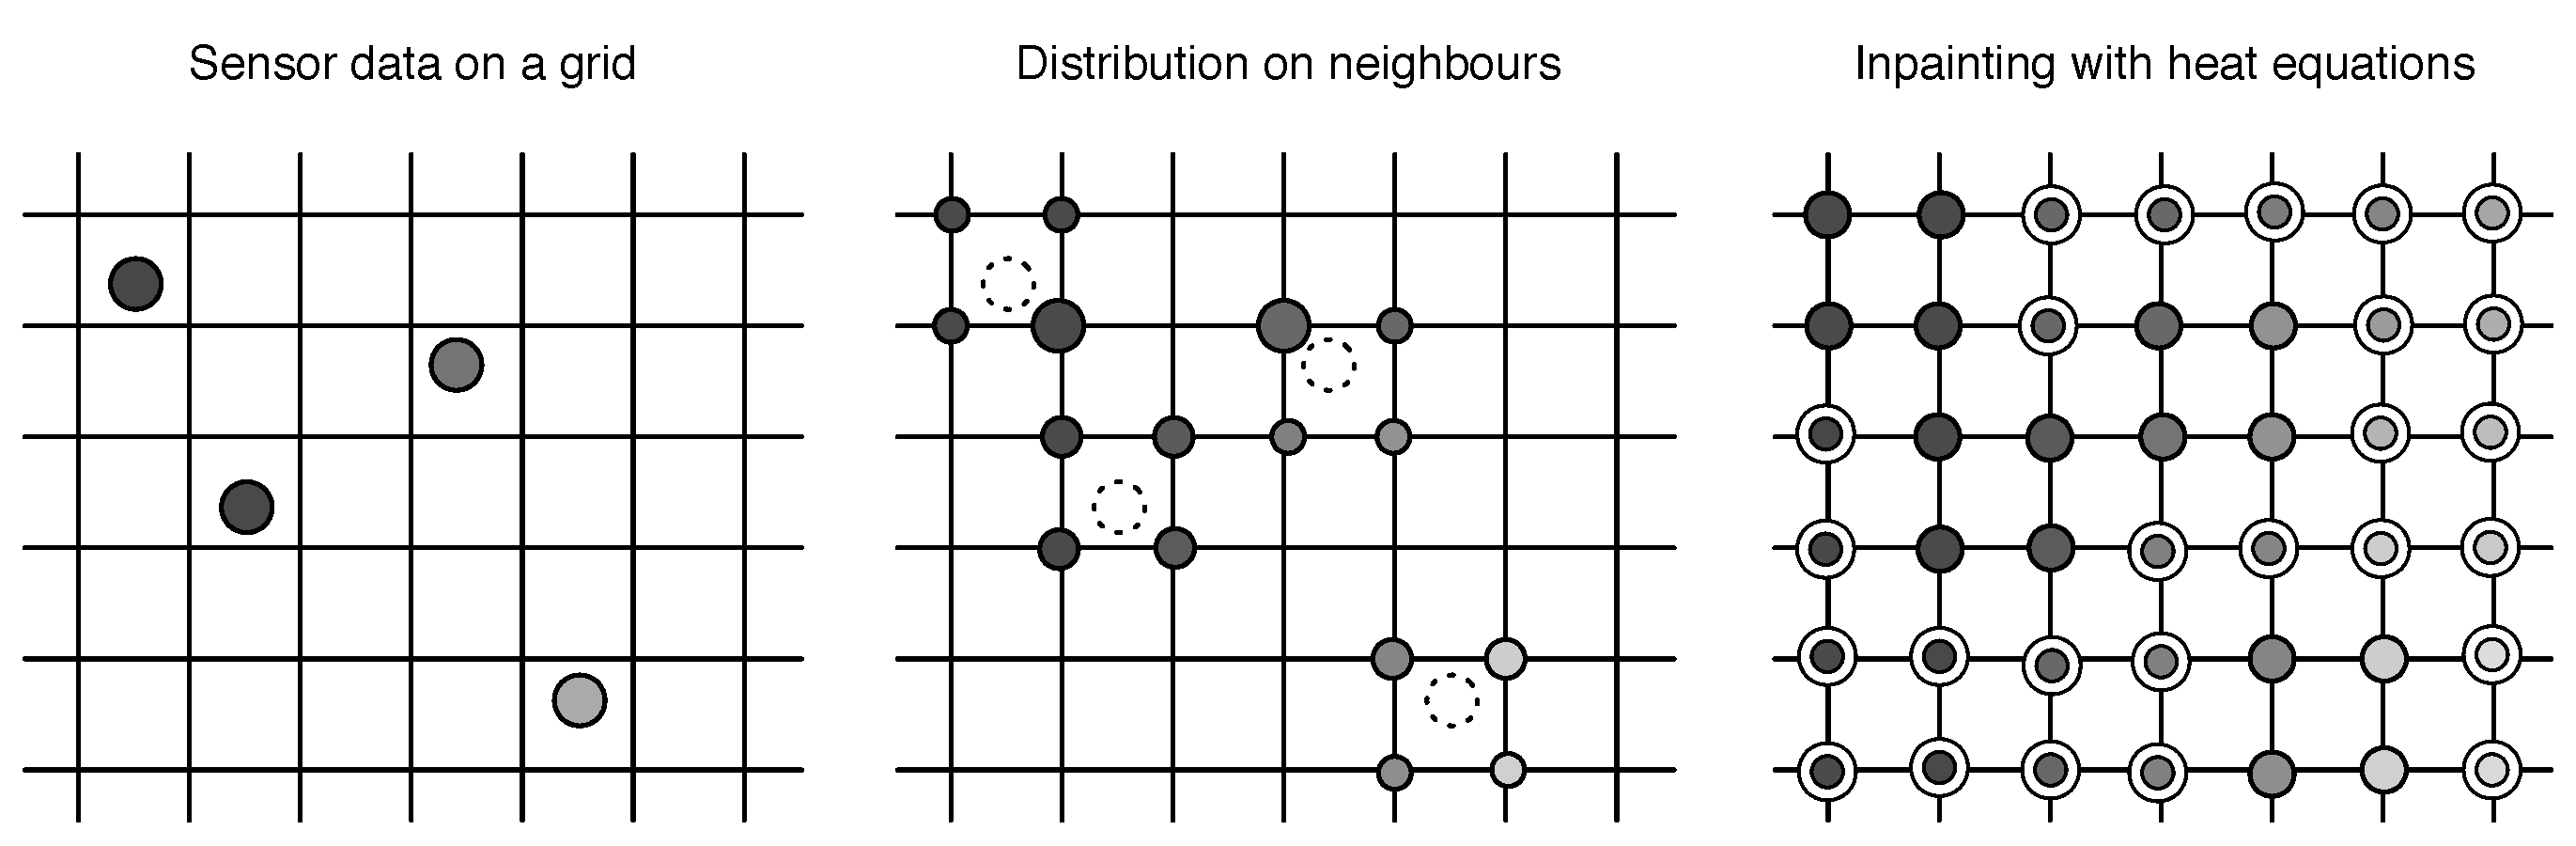
\includegraphics[scale=0.3]{images/inpainting3step.eps}
    \caption{The first image shows that we don't have enough informations to fill out all the pixels. We need to project the data on the neighbours. Finally, the heat equation inpainting will spread the weighted data on the missing spots.}
  \label{inpainting3step}
\end{figure}

Literature shows that heat equations are powerful to fill out these patches of missing data, but it smooths data on sharp edges(high frequency data)\cite{aubert2006mathematical} . One of the effect is that edges are blurred out by the algorithm.


\subsection{OpenGL}

In this section, we see how to render images with OpenGL(Open Graphics Library). It is an API (Application Programming Interface) developed by Silicon Graphics to hide the complexities of interfacing with different 3D accelerators and mainly used for 3D modeling in video games and simulations. OpenGL leverages the fact that GPUs are designed to render triangle. It optimizes the rendering by using the repetition of a geometric shape (tessellation). The more complex the shape the harder it will be for the GPU to process it. If we already pre-process the data into triangles, we minimize processing costs. \cite{abobegpu}

The flow of our program is described by the Fig ~\ref{fig:timelinerendering}. First, we take the X, Y, Z data and generate a list of triplets of points (triangles). Then, we render this list with OpenGL. We will see two methods to render to list of triplets: immediate mode and Vertex Buffer Objects.

\begin{figure}[!ht]
  \centering
  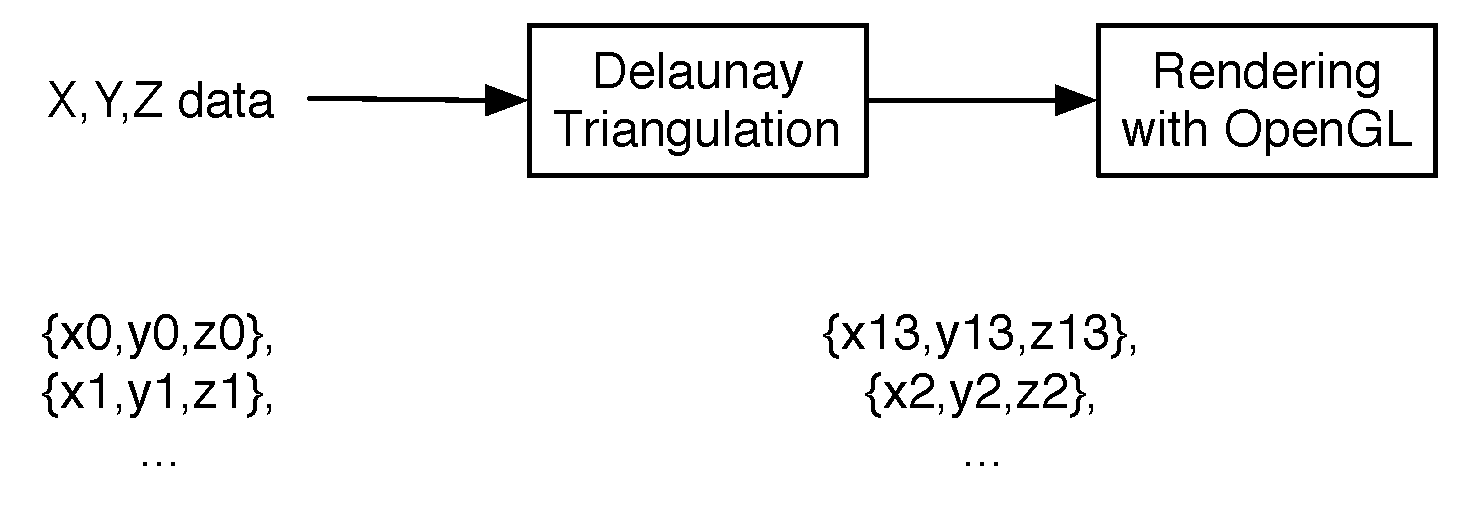
\includegraphics[scale=0.40]{images/timelinerendering.eps}
    \caption{The }
  \label{fig:timelinerendering}
\end{figure}


\subsubsection{Triangulation with Delaunay}

The first problems we face how to generate triangles from sparse data. Indeed, OpenGL can only render triangles from a triplet of points. If we render the X, Y, Z data without preprocessing, OpenGL will generate triplets from the closest index in the list. We need efficient algorithms like Delaunay triangulation to take into account the X, Y position of the point and not the index.

The algorithm minimizes the angles of each triangle. The triangulation is successful if no vertex (i.e. 3-dimensional point) is inside a triangle.

Jonathan Shewchuk \cite{shewchuk96b} has developed a library, triangle.c, to compute Delaunay triangulations and other meshes. The Figure ~\ref{triangulation2d} shows the effect of the program on a spiral scan.  We will discuss later about spiral scanning. The input data has 20'000 points and the program generates 38'784 triangles. 
\begin{figure}[!ht]
  \centering
  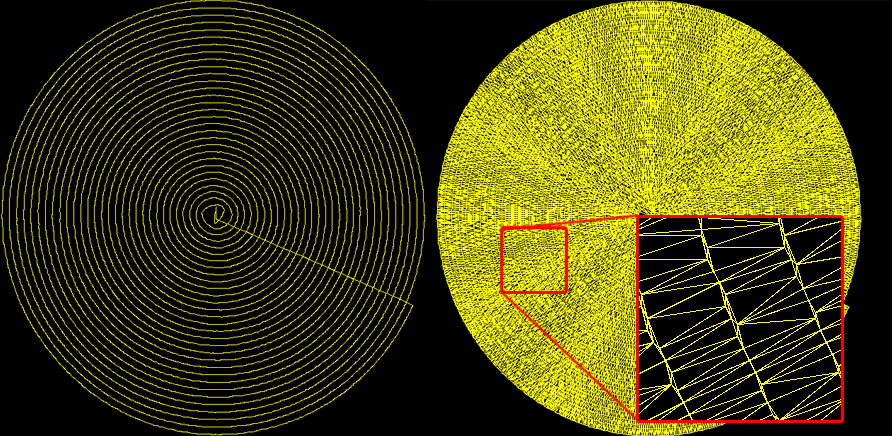
\includegraphics[scale=0.45]{images/triangulation.png}
    \caption{Before and after triangulation. This image is rendered by using the triangle.c library.}
  \label{triangulation2d}
\end{figure}

With this method we can connect the points on a 2D plane. In the figure  ~\ref{triangulation3d}, we use the z-axis data to compute the height of each of our point and render 3D models of our scans. To add colors to our data, OpenGL will create a linear gradient between each of the data points.

\begin{figure}[!ht]
  \centering
  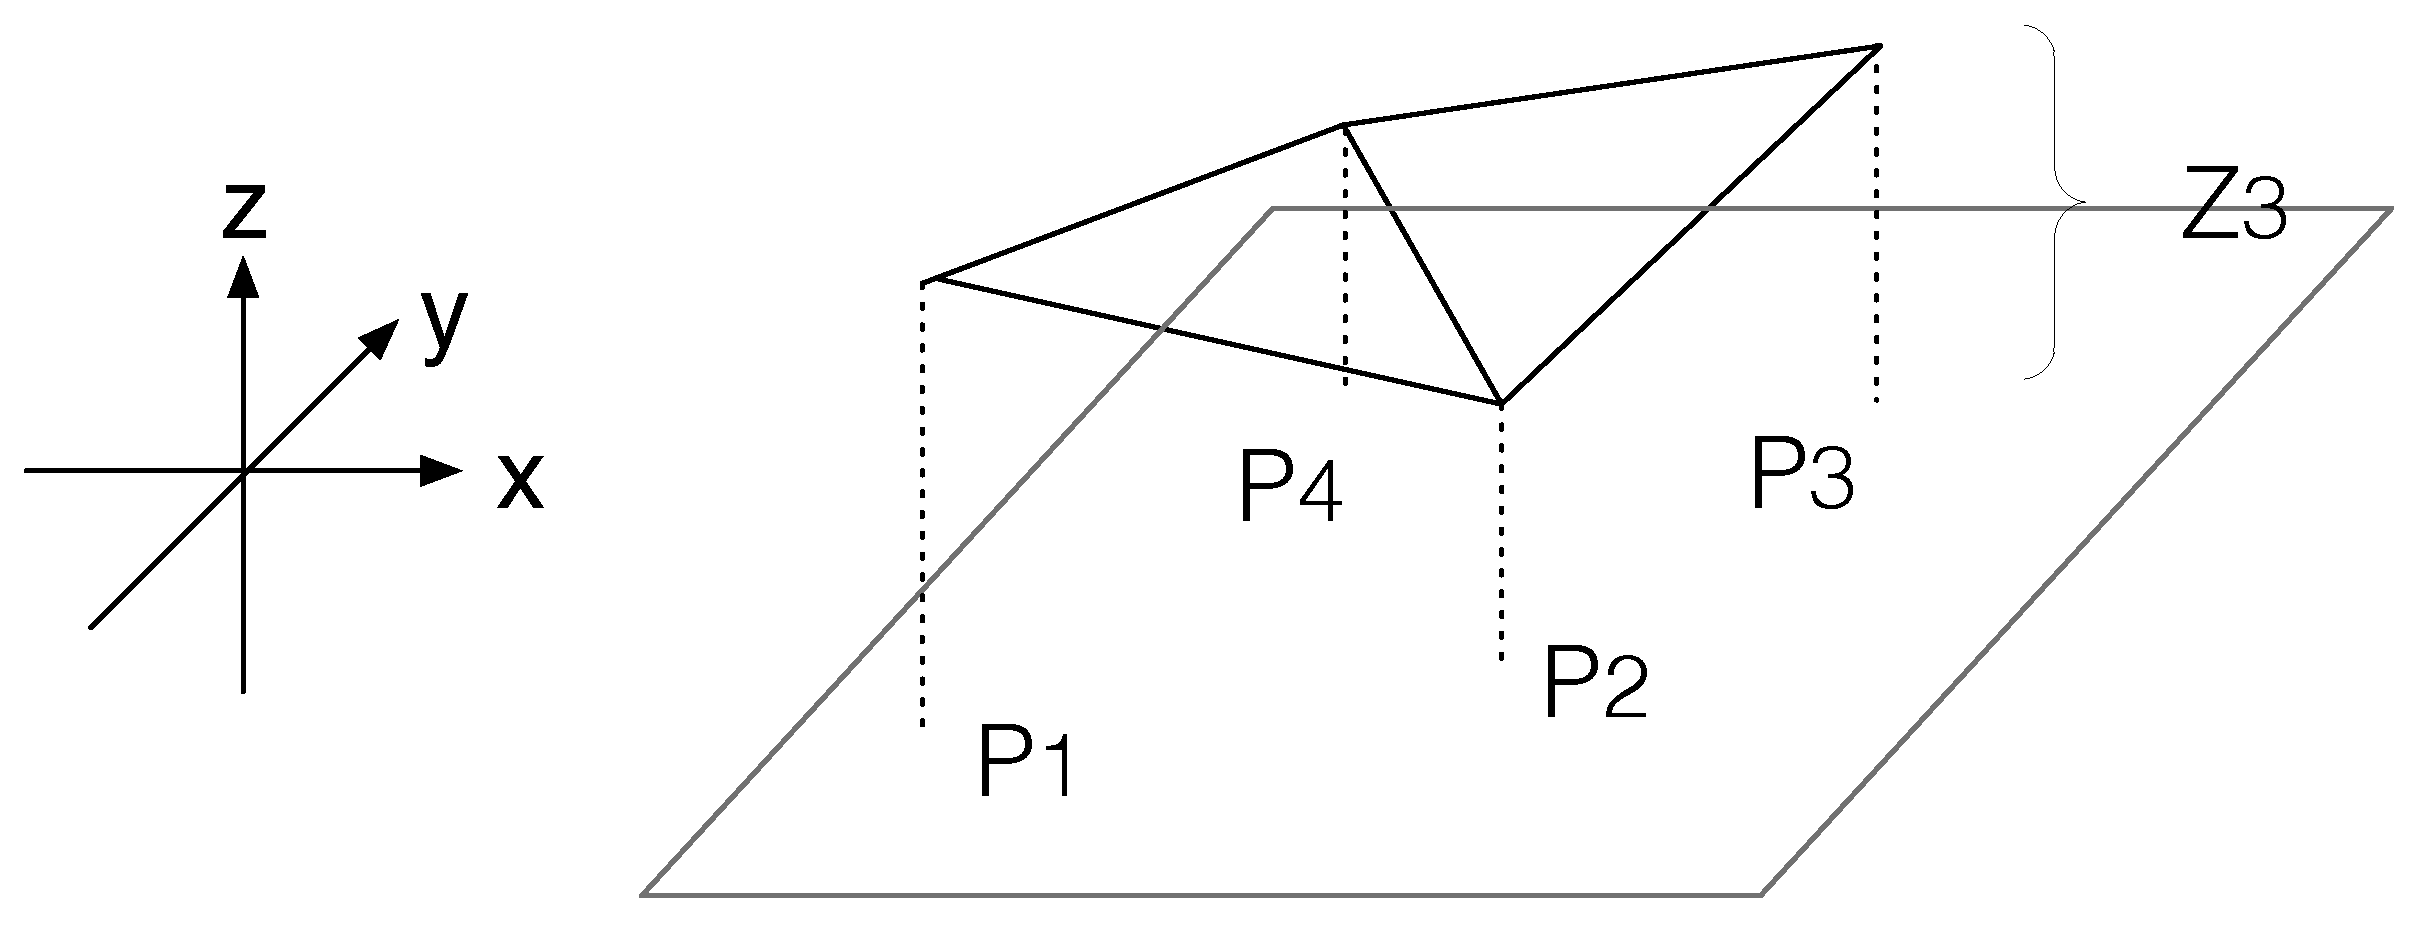
\includegraphics[scale=0.2]{images/delaunay.eps}
    \caption{Delaunay triangulation: From 2D to 3D}
  \label{triangulation3d}
\end{figure}

\begin{figure}[!ht]
  \centering
  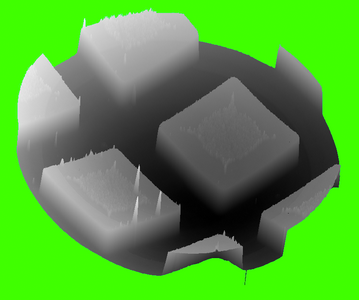
\includegraphics[scale=0.8]{images/3drendering.png}
    \caption{3d rending of 1.2M points}
  \label{rendering3d}
\end{figure}

\subsubsection{Immediate mode vs Vertex Buffer Objects}

There are two ways to render our surface with OpenGL: the immediate mode and vertex buffer objects.

The immediate mode is the simplest implementation of OpenGL. Indeed, we render every frame. If we rotate the our 3D model, we'll have to regenerate the latter. The power of the immediate mode is its simple implementation (no initialization and extra code). Moreover, it is easier to debug. For a small number of vertices (< 10'000) the immediate mode is appropriate. \cite{opengl1} states that the immediate mode is more convenient and less overhead than other implementations (Vertex Buffer Objects).

The display function is called when GLUT(OpenGL Utility Toolkit) determines that the windows needs to be redisplayed. Action like rotation, translation or resizing of the model will trigger the display event. Each time the display function will be called, the program will upload the vertices to the GPU.

If we try to display a significant number of triangles (> 10'000 vertices), the CPU will be the bottleneck. The GPU doesn't start rendering data before the last callback ($glEnd()$). Thus, the CPU is spoon-feeding the GPU by transferring the data triangle by triangle. Moreover, the number of API calls is proportional to the number of triangles. I.e. if you have 10 triangles you will make (10*(2+3+3)) 80 API calls \cite{opengllegacy}. In conclusion, if you want to render less than 10'000 vertices, code a quick implementation and are not planning on making a lot of changes in your rendering, the immediate mode is the way to go.

One of the problem we have encountered with the immediate mode is the transfer from the system memory to the GPU.  We've seen there is a bottle neck in the transfer. With 10'000 points we can only have 3 frames per seconds. It means that our computer takes 300 ms for the whole process.

Instead of transferring the data from the memory to the GPU, the GPU could read the memory of the program. Buffer objects have been created to allow the GPU to have access to the memory. The process of reading the memory from the GPU is called Direct Memory Access (DMA). A buffer object is a contiguous untyped memory which the CPU and the GPU have access to.

We can't just upload our data into the memory without any structure. We need to map the data and make it readable for the GPU. We store our data in a vertex array object.


\begin{figure}[H]
  \centering
  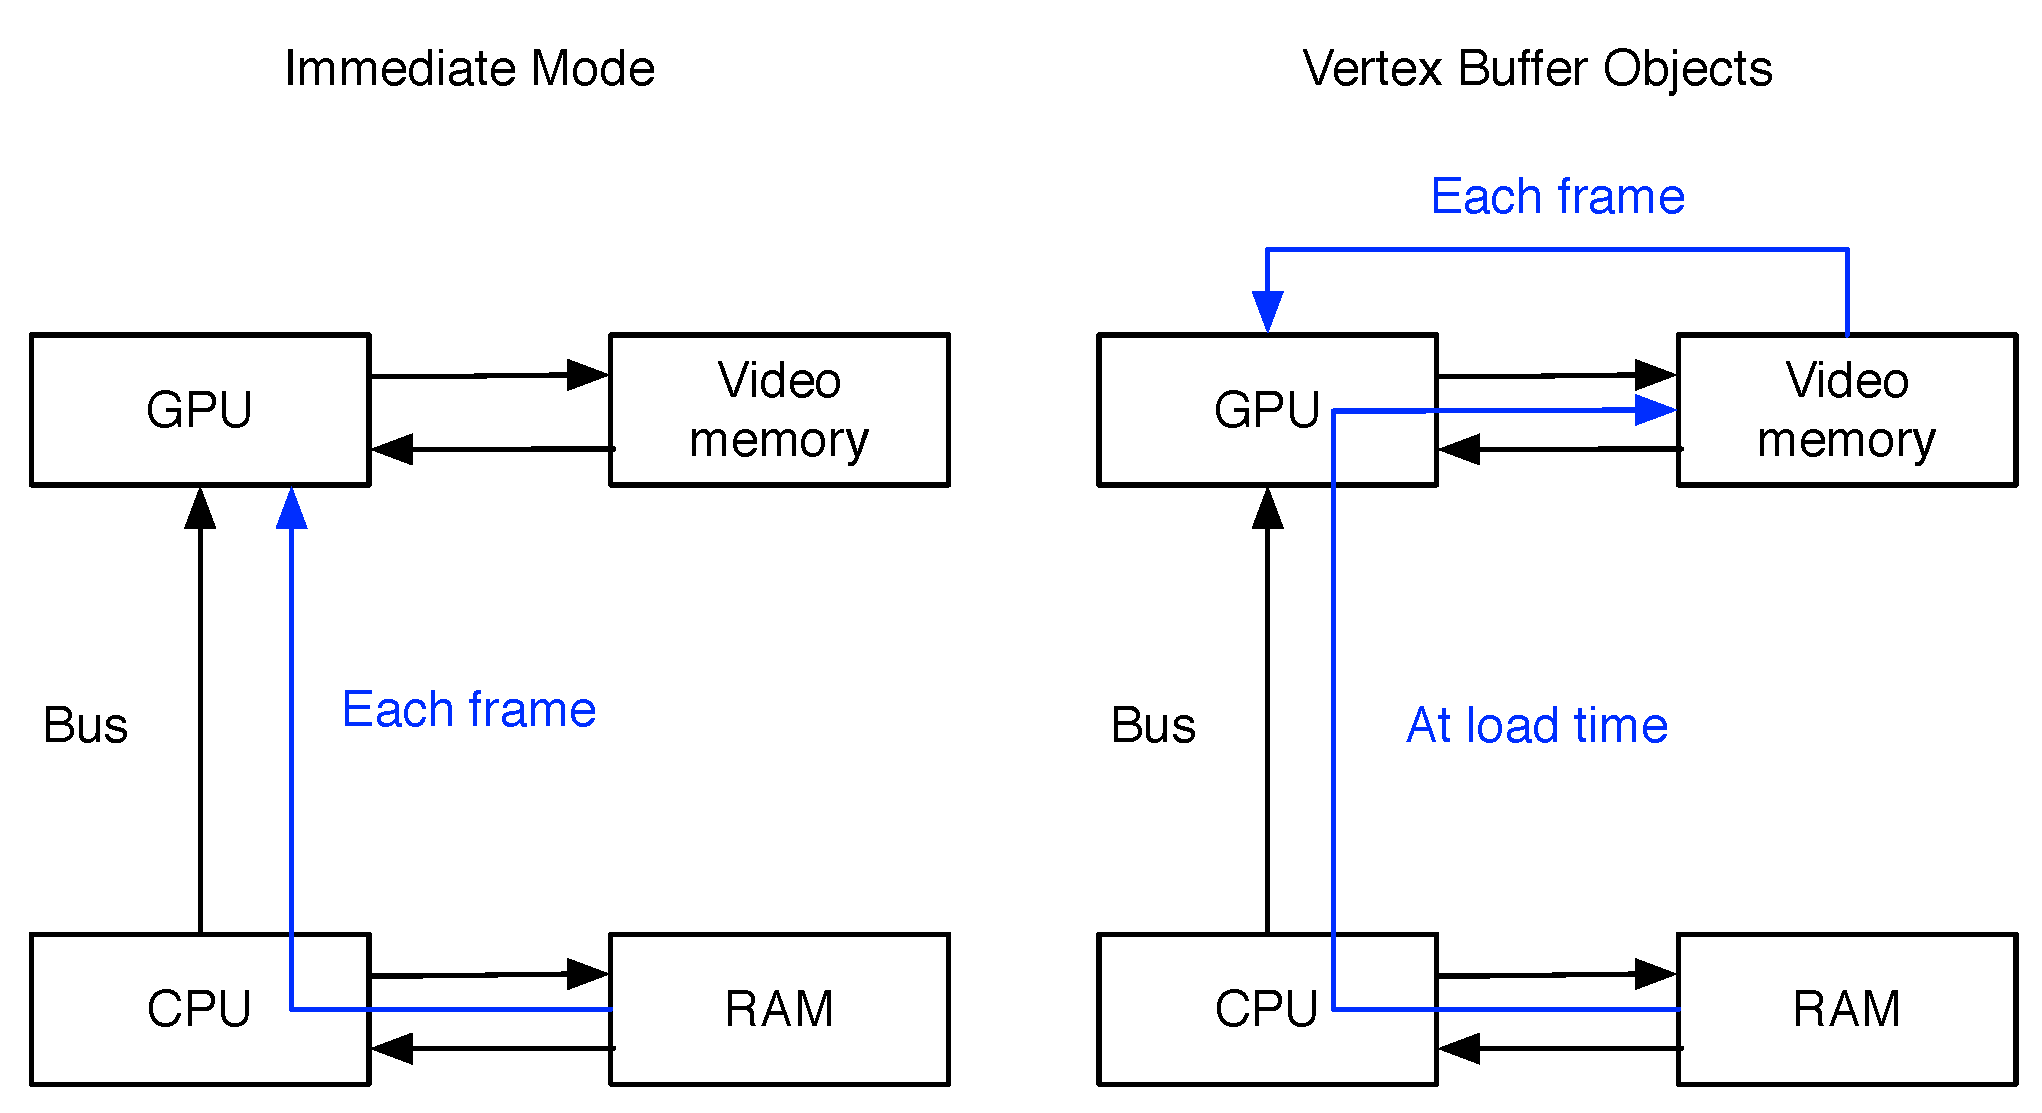
\includegraphics[scale=0.4]{images/openglVBO.eps}
    \caption{Workflow of the immediate mode and the vertex buffer objects}
  \label{openglVBO}
\end{figure}

After having allocated and created this chunk of data, we need to map it to make it readable to the GPU. OpenGL has API calls for that application.

The advantage of this implementation is that you directly pull your data to a shared memory between the CPU and the GPU. Your CPU will spend less cycles making API calls thus improving the performances of the program. The power of the VBOs is that you just need to upload your data and your display function will just bind the VBO. Our performances have improved from 3FPS to 130FPS for 100'000 data points. Having a higher FPS count makes the animations smoother.

Table  ~\ref{table:nonlin} shows the non-linearity of our implementation. We see that Delaunay triangulation doesn't scale well for 1'000'000 points. In AFM scans we will rarely sample 1'000'000 datapoints. The limits of our AFM is 100'000 kHz. If we take 10 seconds scans at the limit rate, we observe that the computation time is still way below the scanning time. 

\begin{table}[ht]
\caption{Rendering results[ms]} % title of Table
\centering % used for centering table
\begin{tabular}{c |c c| c } % centered columns (4 columns)
\hline\hline %inserts double horizontal lines
 Nb of points & Delaunay & VBO & Total time\\ [0.5ex] % inserts table 
%heading
\hline % inserts single horizontal line

1000 & 2.9 & 23.9 & 26.8 \\
10000 & 8.1	&	27 	& 35.1\\
100000 & 66.9 & 181 & 247.9 \\
1000000 & 640.7	& 267 & 907.7\\[1ex]


\hline %inserts single line
\end{tabular}
\label{table:nonlin} % is used to refer this table in the text
\end{table}


